\documentclass[12pt,a4paper]{article}
\usepackage{lmodern}
\usepackage[utf8]{inputenc}
\usepackage[T1]{fontenc}
\usepackage{geometry}
\usepackage{setspace}
\usepackage{graphicx}
\geometry{a4paper, total={170mm,257mm}, left=20mm, top=20mm}

\title{\Huge BaDMat 1.0 \\ \LARGE Mode d'emploi} % Ça fait un peu BatMan, on garde vraiment ce nom-là ?
\author{Myrtille Grulois \thanks{Université populaire et citoyenne de Roubaix}}
\date{Été 2020}

\renewcommand*\contentsname{Sommaire}

\begin{document}

\begin{titlepage}
\maketitle
\end{titlepage}

\tableofcontents
\clearpage

\addcontentsline{toc}{section}{Introduction}
\section*{Introduction}

Ce manuel d'utilisation concerne la première version du logiciel BaDMat de l'UPC de Roubaix.
Les explications concernent à la fois la structure de la base de donées et les différentes fonctions disponibles.
Pour toute action d'ordre général, se reporter au préambule, qui contient des instructions valables pour la plupart des fonctions (sauf mention contraire).

\bigskip
\section{Préambule : ce qu'il est utile de savoir (faire)}

\subsection{Ouverture du terminal}

    Bon je vais pas trop détailler, comme on n'a pas encore décidé de l'OS à utiliser\dots
    À mettre à jour.


\bigskip
\subsection{Lancement d'un script}
    Tout d'abord, précisons que dans notre cas, un script correspond à une fonctionnalité.
    Chaque fonction décrite ci-dessous est donc lancée à partir d'un fichier différent.
    Pour lancer un script (à compléter, dépend 1. de l'OS 2. de comment fonctionne Python sur l'OS)


\bigskip
\subsection{Utilisateurs et connexion à la base de données}
    À compléter une fois qu'on aura discuté des mots de passe
    Préciser que c'est normal si on ne voit pas le mdp qui s'affiche quand on tape.

\bigskip
\subsection{Interactions avec le programme}
    Pour la plupart des instructions, le programme nécessite que vous rentriez une lettre en majuscule.
    Tapez la lettre correspondant à votre choix parmi les propositions de la question,
    puis validez en tapant "Entrée".


\bigskip    
\subsection{Définition des termes utilisés}
    On parlera plus loin de table lorsqu'on parlera de catégorie : ainsi, il y aura par exemple
    une table pour les différents matériaux, et une autre pour les pièces qui sont composées de ces matériaux.

    Tout au long de la suite, ligne désignera une entrée dans la base de données.
    Colonne désignera un des possibles critères de cette ligne.
    
    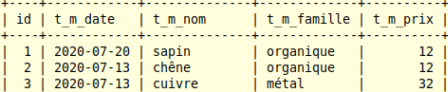
\includegraphics{exemple_lignes_colonnes.png}

    Dans l'exemple ci-dessus, vous avez un extrait de la table des matériaux.
    Une ligne de cette table (par exemple celle d'ID 1 décrivant le sapin) correspond à une entrée
    dans la table, donc à un matériau. Elle sera nommée\dots ligne.
    On nommera colonne, par exemple, le critère ID. Pour aller plus loin, la colonne ID
    est de type numérique, tandis que la colonne t\_m\_famille est de type textuel.
    Reportez-vous à la section \textbf{Structure de la base de données} pour connaître plus précisément
    les types de chaque colonne.



\clearpage
\section{Fonctions}

Cette section regroupe les différentes fonctions implémentées, ainsi que la façon de les exécuter, et les différentes options possibles.

\bigskip
\subsection{Recherche}

    La fonction principale de cette base de données est la fonction de recherche.
    Pour l'exécuter, lancer le script \emph{search.py}, puis se connecter à la base de données.
    Vous devrez commencer par choisir dans quelle table est-ce que la recherche s'effectuera.
    Il existe deux types de recherche : la recherche simple et la recheche avancée.

    \subsubsection{Recherche simple}
        La recherche simple est à privilégier si vous ne souhaitez inclure qu'une seule colonne dans votre recherche.
        Vous aurez toujours la possibilité de choisir quelle(s) colonne(s) vous souhaitez afficher dans les résultats.


        \medskip
        \textbf{Recherche textuelle}

        Si la colonne que vous sélectionnez est de type textuel, alors vous pourrez entrer un mot ou une expression.
        
        \medskip
        \textbf{Recherche numérique}
        
        Si la colonne que vous sélectionnez est de type numérique, vous pourrez effectuer une recherche autour d'une valeur donnée,
        ou bien une recherche sur un intervalle. Si vous choisissez la recherche numérique simple, vous aurez toutefois
        la possibilité d'entrer une tolérance. La recherche s'effectuera alors sur l'intervalle de longueur de deux fois votre tolérance
        qui entoure votre valeur.

        \medskip
        \textbf{Recherche par date}
        
        Vous pouvez également effectuer une recherche sur la date.

    \subsubsection{Recherche avancée}
        La recherche avancée vous prendra plus de temps. Elle permet à la fois d'effectuer une recherche sur plusieurs colonnes,
        mais également de rechercher plusieurs critères dans la même colonne (pour les colonnes de texte).

        \medskip
        \textbf{Recherche textuelle}

        Si la colonne que vous sélectionnez est de type textuel, alors vous pourrez entrer un mot ou une expression, qui sera recherché
        dans cette colonne. Toutefois, vous aurez ensuite la possibilité d'ajouter des mots supplémentaires, que vous pourrez moduler :
        c'est-à-dire imposer que le mot saisi ne se trouve pas dans les résultats de votre recherche, ou bien cherche le premier terme
        ou bien le deuxième, etc.
        
        \medskip
        \textbf{Recherche numérique}
        
        La recherche numérique avancée est identique à celle de la recherche simplifiée.
        Si la colonne que vous sélectionnez est de type numérique, vous pourrez effectuer une recherche autour d'une valeur donnée,
        ou bien une recherche sur un intervalle. Si vous choisissez la recherche numérique simple, vous aurez toutefois
        la possibilité d'entrer une tolérance. La recherche s'effectuera alors sur l'intervalle de longueur de deux fois votre tolérance
        qui entoure votre valeur.

        \medskip
        \textbf{Recherche par date}
        
        Vous pouvez également effectuer une recherche sur la date.


\bigskip
\subsection{Ajouter une nouvelle ligne}

    Lorsque vous souhaitez ajouter une nouvelle ligne, il vous faut utiliser le script \emph{addRow.py}.
    Connectez-vous, puis indiquez quelle table vous souhaitez compléter.
    On vous demandera ensuite d'entrer un par un les critères que vous souhaitez compléter.
    Si pour un critère donné vous ne savez pas, vous pouvez simplement taper "Entrée".
    Cela laissera vide la colonne concernée.
    Toutefois, certaines colonnes ne peuvent pas être laissées vides. Pour celles-là (plus de précisions dans
    la section \textbf{Structure de la base de données}), il faut impérativement que vous entriez une valeur.

    La complétion de certaines colonnes est conditionnée par des termes préalablement rentrés. Par exemple,
    il ne vous est pas possible d'entrer une pièce composée d'un matériau qui n'est pas présent dans la base
    de données. Il faudra d'abord que vous créiez le matériau, puis vous pourrez ajouter la pièce associée.
    Le même principe s'applique pour la famille de matériaux. Un certain nombre de termes est autorisé (organique,
    métal, alliage, composite, polymère, céramique). Si vous essayez de rentrer un autre terme, vous obtiendrez une
    erreur. La liste complète des colonnes contraintes et des termes autorisés est consultable dans la section
    \textbf{Structure de la base de données}.


\bigskip
\subsection{Modifier une ligne existante}
    
    Utilisez pour cela le script \emph{modifyRow.py}.
    Après vous être connecté et avoir sélectionné la table sur laquelle vous souhaitez travailler,
    il faut que vous connaissiez l'ID exact de la ligne à modifier. Si ce n'est pas le cas,
    commencez plutôt par effectuer une recherche, dans laquelle vous sélectionnerez la colonne ID
    parmi les colonnes à afficher.

    Modifier une ligne se passe à peu près comme pour en ajouter une. On vous propose tous les critères
    un par un, à vous de les compléter.


\bigskip
\subsection{Supprimer une ligne existante}

    Le script à utiliser est le script \emph{delete.py}.
    Après connexion et choix de la table, il vous faudra, là encore, renseigner l'ID exact de la ligne
    à supprimer.


\bigskip
\subsection{Fusionner deux lignes existantes}

    Utilisez pour cela le script \emph{merge.py}.
    Connectez-vous et choisissez la table. Bien entendu, vous ne pouvez fusionner deux lignes
    que si elles se trouvent dans la même table. Vous aurez besoin des ID des deux lignes à fusionner.
    
    Le programme vous proposera automatiquement une possibilité de fusion. Pour celle-là, il privilégiera
    de remplir au maximum les colonnes, et, en cas de doute, de conserver la valeur de la ligne dont vous
    aurez donné l'ID en premier.
    Ainsi, si les deux valeurs sont identiques, il vous proposera automatiquement cette valeur. Si l'une
    des lignes n'est pas remplie, il suggérera automatiquement l'autre valeur. En cas de remplissage différent
    pour les deux lignes, il vous proposera par défaut la valeur présente sur la première ligne. Vous verrez
    entre parenthèses la valeur que contenait la deuxième ligne.

    Si vous souhaitez modifier la valeur proposée par défaut (que ce soit pour la remplacer par la valeur
    entre parenthèses ou par une autre valeur), il vous suffit de taper la valeur de remplacement et de saisir
    "Entrée".


\bigskip
\subsection{Sauvegarde et restauration de la base de données}
    
    Il est conseillé d'effectuer régulièrement des sauvegardes de la base de données.
    Pour cela, utilisez le script \emph{backup.py}. Vous ne pouvez enregistrer qu'une seule sauvegarde
    chaque jour, puisque le programme utilise pour cela la date. Faites donc attention : il est conseillé d'effectuer
    une sauvegarde préalable avant toute altération de la base de données, a fortiori s'il s'agit de suppression,
    de fusion ou de modification, puisque ces opérations écrasent définitivement les données précédentes, et ne sont
    pas récupérables autrement que grâce à cette backup.

    Vous pouvez utiliser le même script pour restaurer une sauvegarde qui a été effectuée récemment. Soit la sauvegarde
    du jour, soit vous pouvez choisir manuellement la date que vous souhaitez.
    Les fichiers de sauvegarde sont des fichiers que vous pouvez consulter avec n'importe quel éditeur de texte.
    Leur structure n'est pas très lisible, mais vous permet tout de même de retrouver certaines informations, si vous
    avez un doute sur la date de la sauvegarde que vous souhaitez restaurer.

    Notez bien que restaurer une sauvegarde permet d'annuler toutes les modifications qui ont été effectuées depuis,
    donc écrase toutes les nouvelles données entrées.


\bigskip
\subsection{Créer la base de données}

    Cette action n'est à effectuer qu'une seule fois, au début.
    Ouvrir le terminal % invite de commande si windows, voir choix os.
    et se connecter à mysql.
    Taper \verb+CREATE DATABASE TestDB;+ et valider. Si la réponse est du
    style \verb+Query OK, 1 row affected (0.00 sec)+, c'est que la requête
    a réussi, et que la base de données est prête à être créée.
    
    Vous pouvez alors exécuter le script \emph{createDB.py}. Ce script va créer
    la base de données avec toutes ses tables et ses colonnes. Toutefois elle
    sera vide, ce sera à vous d'y ajouter des lignes.

    Si vous avez récupéré une sauvegarde et que vous souhaitez donc compléter
    automatiquement les tables lors de la création de la base de données, vous
    préférerez utiliser le script \emph{backup.py}.


\clearpage
\section{Base de données}

\bigskip
\subsection{Structure de la base de données}

\begin{verbatim}
    Test de code Blablabla
    Deuxième ligen
    Là je laisse une indentation
    for i in range(0, 3):
\end{verbatim}


\end{document}